\section{Modernien anturiverkkojen tiedonsiirto-ongelmat}

Anturiverkkojen toimintaolosuhteista johtuen verkon yhteydet ovat muuttuvia ja
ennalta-arvaamattomia. Usein verkon yksittäisillä antureilla ei ole tietoa
verkon koostumuksesta sen välittömien naapureiden lisäksi. Siksi
reititysprotokollien täytyy pystyä sopeutumaan muuttuviin tilanteisiin
mahdollisimman vähällä informaatiolla itse verkosta.

Ensimmäinen artikkeli keskittyy anturiverkkojen keräämän datan tehokkaaseen
yhdistämiseen, eli datafuusioon. Toinen taas pyrkii kehittämään
reititysprotokollan joka on robusti ja pystyy mukautumaan antureiden
tuhoutumisesta johtuviin muutoksiin.

\subsection{Datafuusio}
Artikkelissa~\cite{Yu2006} keskeistä on anturien keräämän datan fuusio.
Datafuusio tarkoittaa toisiinsa liittyvän datan liittämistä yhteen. Artikkeli
käyttää esimerkkinä UAV:sta koostuvaa anturiverkkoa, joissa jokaisella
yksittäisellä UAV:lla on matala varmuus kokonaistilanteesta. Datafuusio on
tärkeää jotta verkolla on vahva käsitys tilanteesta jonka avulla se voi
suunnitella toimintaansa.

Datafuusio toimii niin että toisiinsa liittyvä data koitetaan kerätä yhteen.
Verkon solmut lähettävät dataa eteenpäin kunnes jollakin solmulla on tarpeeksi
paljon dataa, jolloin se lopettaa datan eteenpäinlähetyksen ja rupeaa
prosessoimaan dataa ja tekemään sen avulla päätöksiä.

\subsection{Luotettava tiedonsiirto anturiverkoissa}
Anturiverkon solmujen kuolemat ovat ongelma jonka verkon täytyy pystyä
kestämään ja käsittelemään. Kuolema tarkoittaa tässä kontekstissa mitä tahansa
tilannetta jossa solmu on toimintakyvytön tai sen toimintakyky on niin huono
että siitä ei ole hyötyä verkossa. Artikkelissa~\cite{Arya2015} esitelty
algoritmi pyrkii etsimään solmujen kuolemista syntyviä ``reikiä'' ja
reitittämään data optimaalisesti ne huomioon ottaen.

% \TODO{Ehkä yksi kappale lisää tähän? Tai jos ei niin sitten yhdistä toiseen
% sektioon}

% \subsection{Muita anturiverkkojen reititysalgoritmeja}
% \TODO{Kerro joistain muista reititysprotokollista, ja siitä miksi ne eivät
% sovellu kuitenkaan tässä esitettyihin ongelmiin}

\section{Vahvistumisoppiminen anturiverkojen tiedonsiirrossa}

Kummatkin artikkelit siis ryhtyvät ratkaisemaan anturiverkkojen tiedonsiirron
reitityksen optimointia. Molemmat myös pyrkivät löytämään nopeita ja
luotettavia yhteyksiä solmujen väleille. Ensimmäinen kuitenkin pyrkii
pääasiassa etsimään verkon reikiä ja toinen pyrkii optimoimaan datafuusiota.

Vahvistusoppimisessa voidaan ajatella olevan kolme komponenttia
\begin{description}
  \item[Agent, toimija] on vahvistusoppimisen opetuksen kohde. Esimerkiksi
    robotti, jonka tulee oppia nopein reitti päämääräänsä.
  \item[Action, toiminta] on jotain mitä toimija voi tehdä. Esimerkiksi ``liiku
    pohjoisessa olevaan huoneeseen''.
  \item[Environment, ympäristö] vaikuttaa toimijan mahdollisiin toimintoihin ja
    niiden onnistumiseen. Toimintojen hyöty voi olla erittäin riippuvainen
    toimintaympäristöstä. Edelliseen esimerkkiin liittyen liikkuminen
    pohjoiseen ei välttämättä ole aina paras toiminto. Pohjoiseen vievä reitti
    voi olla esimerkiksi umpikuja.
\end{description}
Kuten kappaleessa~\ref{sec:terms} jo sanottiin, vahvistusoppimisessa oppijan,
eli toimijan, tulee löytää ympäristössään optimaalinen toiminta. Se löytää, tai
oppii tämän optimaalisen toiminnan kokeilemalla eri toimintoja. Tehdessään
toiminnon, se saa siitä jollain tavalla palautetta, joka vaikuttaa siihen minkä
toiminnon se valitsee ensi kerralla; Jos palaute oli positiivista, se valitsee
saman toiminnon. Jos taas negatiivista, se luultavasti kokeilee muuta
toimintoa.

``Q-learning'' tai Q-oppiminen on yksi vahvistusoppimisen menetelmä. Menetelmä
ei vaadi tarkkaa mallia ympäristöstä, ja siten soveltuu lähes mihin tahansa
vahvistusoppimisongelmaan.  Q-oppimisessa toimijan potentiaalisilla
toiminnoilla toimitaympäristössään on joku hyöty, eli Q-arvo. Kriittistä
Q-oppimisessa on Q-arvon päivittäminen toiminnasta saadun palautteen avulla;
Tämä on menetelmän tapa oppia optimaalinen toimintatapa ympäristössä.
Q-oppiminen pyrkii ottamaan huomioon myös ajan. Ajan huomioiminen on tärkeää
koska varsinkin reaalimaailmassa useimmat toiminnot eivät ole heti palkitsevia,
vaan ne mahdollistavat tulevaisuudessa toimintoja jotka ovat arvokkaita.
Toiminnan lopullinen hinta määräytyy siis nykyisen tilan lisäksi tiloista
joihin toiminto johtaa.~\parencite{Kaelbling1996}

\subsection{Datan tehokas yhdistäminen vahvistusoppimisen avulla}

Yksinkertainen algoritmi datan yhdistämiseen anturiverkossa on niin sanottu
``path reinforcement'' algoritmi, jonka toimintaa havainnollistaa
kuva~\ref{fig:yu2006}. Kun algoritmi ensimmäisen kerran saa dataa tietystä
tapahtumasta, se lähettää sen satunnaiselle naapurille eteenpäin. Kun se saa
samasta tapahtumasta lisää dataa, se lähettää sen eteenpäin sille naapurille
jolle se viimeksi lähetti dataa kyseisestä tapahtumasta.  Tapahtuman ja datan
samankaltaisuuden tai liittyvyyden määrittely on oma ongelmansa johon
artikkelissa~\cite{Yu2006} ei oteta kantaa. Algoritmin ideana on että jos data
reititetään aina samaa reittiä pitkin, todennäköisyys että jollekin reitin
solmulle tulee tarpeeksi dataa kasvaa.

\begin{figure}[h]
  \centering
  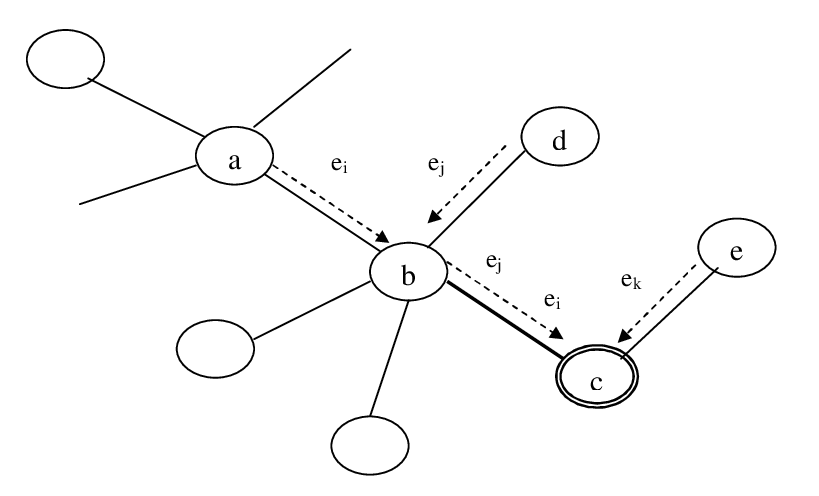
\includegraphics[width=0.8\linewidth]{yu2006_kuva}
  \caption{Havainnekuva siitä kuinka ``path reinforcement'' algoritmi pyrkii
    lähettämään toisiinsa liittyvän datan samalle solmulle.~\parencite{Yu2006}}
\label{fig:yu2006}
\end{figure}

Vaikka kyseinen algoritmi edistää datafuusiota melko tehokkaasti ilman kattavaa
tietoa anturiverkosta, sen ongelmana on että se ei ota huomioon verkon
yhteyksien laatua, tai edes sitä meneekö tieto perille. Eli se pyrkii
lähettämään dataa samalle naapurille vaikka yhteys olisi huono tai jopa
olematon. Ongelma voidaan korjata lähettämällä data uudestaan jos vikoja tai
huonoja yhteyksia havaitaan verkossa. Uudelleenlähetys kuitenkin laskee
algoritmin tehokkuutta melko paljon, koska uuden naapurin valinta on
satunnaista jolloin data saatetaan lähettää uudestaan vialliselle naapurille,
tai muuten epäoptimaaliselle naapurille.

Tehokkuutta voidaan parantaa mallintamalla naapureiden luotettavuutta jollain
tavalla. Tässä päästäänkin artikkelin~\cite{Yu2006} keskeiseen algoritmiin,
jota tekijät itse kutsuvat ``path learning'' algoritmiksi. Perusidea datan
yhdistämisen kannalta on sama kuin path reinforcementissa; Samankaltainen data
pyritään reitittämään samaa reittiä pitkin, jotta todennäköisyys että data
päätyy samalle solmulle on korkeampi. Algoritmi käyttää kuitenkin
vahvistusoppimista hyväkseen opettemalla solmuille toiminnan myötä mitkä
naapurit pystyvät luotettavimmin lähettämään dataa myös eteenpäin.

Artikkelissa~\cite{Yu2006} tehtyjen simuulatioiden perusteella kyseinen
algoritmi parhaimmillaan kaksinkertaistaa datafuusion todennäköisyyden
verrattuna ``random walks'' algoritmiin, jossa vastaanottaja siis valitaan
satunnaisesti. Algoritmi kestää myös hyvin solmujen tuhoutumista; Tilanteessa
jossa jopa 50\% solmuista tuhoutui, datafuusion todennäköisyys oli 70\%.

\subsection{Vahvistusoppimisen hyödyntäminen sopeutuvassa anturiverkossa}

Kuten datafuusiossa, myös artikkelissa~\cite{Arya2015} käytetään hyväksi
vahvistusoppimista tehokkaan reititysprotokollan luomiseksi. Kuten datafuusioon
keskittyvän algoritmin kanssa, sopeutuvan reitityksen algoritmi pyrkii
huomioimaan solmun naapureiden luotettavuutta. Kyseinen algoritmi ottaa
kuitenkin myös huomioon muita muuttujia, kuten vastaanottajan akkutilanteen.
Lisäksi tässä algoritmissa otetaan huomioon koko reitti päämäärään asti, ei
ainoastaan hyppy naapurille. Myös tässä algoritmissa vastaanottajan ``hyvyys''
määräytyy sen antaman palautteen mukaan. Yhden solmun oppiminen voidaan siis
kuvata tapahtumaketjuna, jossa se
\begin{enumerate}
  \item Valitsee naapureistaan vastaanottajan niiden Q-arvon perusteella
  \item Lähettää datan eteenpäin valitulle naapurille
  \item Päivittää naapurin Q-arvon siltä saadun palautteen perusteella
\end{enumerate}
Kuvassa~\ref{fig:arya2015_oppiminen} on yksinkertainen
systeemikuva~\cite{Arya2015} kuvaaman vahvitusoppimista käyttävän algoritmin
toiminnasta.

Luotettavan reitityksen lisäksi kyseisen algoritmin keskeisiä päämääriä on
tunnistaa reiät anturiverkon kattavuudessa. Reiät kattavuudessa syntyvät kun
antureita vioittuu tai ne eivät jostain muusta syystä pysty keräämään tai
reitittämään dataa tarpeeksi hyvin. Tämän seurauksena verkkoon muodostuu
``reikä'', jonka läpi ei voi lähettää dataa, vaan tiedonsiirron täytyy mukautua
sen ympärille. Reiän havaitseminen on siis tärkeää optimaalisen reitityksen
kannalta. Useimmissa anturiverkon sovelluksissa on myös erittäin hyödyllistä
olla tietoinen miltä alueilta ei saada tietoa; Myös tämän takia on tärkeää
havaita verkon reiät.

Jotta reikiä voidaan löytää täytyy ensin etsiä optimaalinen reititys olemassa
olevalle verkolle. Tämä tapahtuu edellä kuvatulla tavalla. Aluksi verkon nielut
myös pyytävät antureita ja muita solmuja lähettämään itsestään dataa verkon
yli, jotta optimaalinen reititys löytyisi mahdollisimman nopeasti; Verkon
reitityshän perustuu vahvistusoppimiseen, joten optimaalista reittiä ei saada
selville ilman että tiedonsiirtoa kokeillaan. Kun optimaalinen reititys on
löydetty, voidaan ruveta havaitsemaan reikiä. Jos solmu itse havaitsee
vioittuneensa se pyrkii lähettämään viestin tilastaan. Tämän viestin avulla sen
naapurit voivat päivittää omat tietonsa kyseisestä solmusta. Tämän lisäksi
tukiasema ajaa säännöllisesti algoritmia jonka on tarkoitus havaita reiät
joista solmut itse eivät ole ilmoittaneet.

\begin{figure}[h]
  \centering
  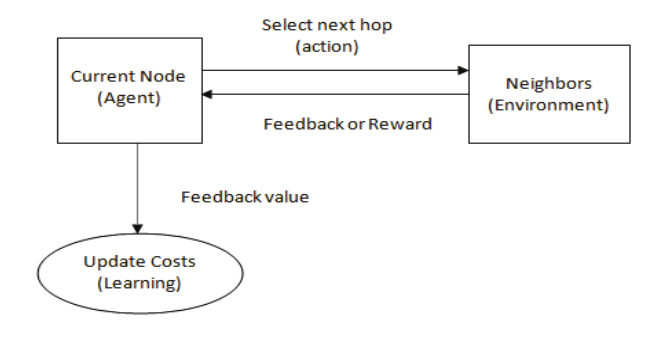
\includegraphics[width=0.8\linewidth]{arya2015_oppiminen}
  \caption{Systeemikuva reititysalgoritmin vahvistusoppimisesta.~\parencite{Arya2015}}
\label{fig:arya2015_oppiminen}
\end{figure}

Artikkelissa on myös simuloitu algoritmin toimintaa ja suorituskykyä.
Kuvassa~\ref{fig:arya2015} näkyy simuloitu tilanne, jossa osa solmuista on
``kuollut''. Kuolleiden solmujen seurauksena syntynyt reikä näkyy mustana.

\begin{figure}[h]
  \centering
  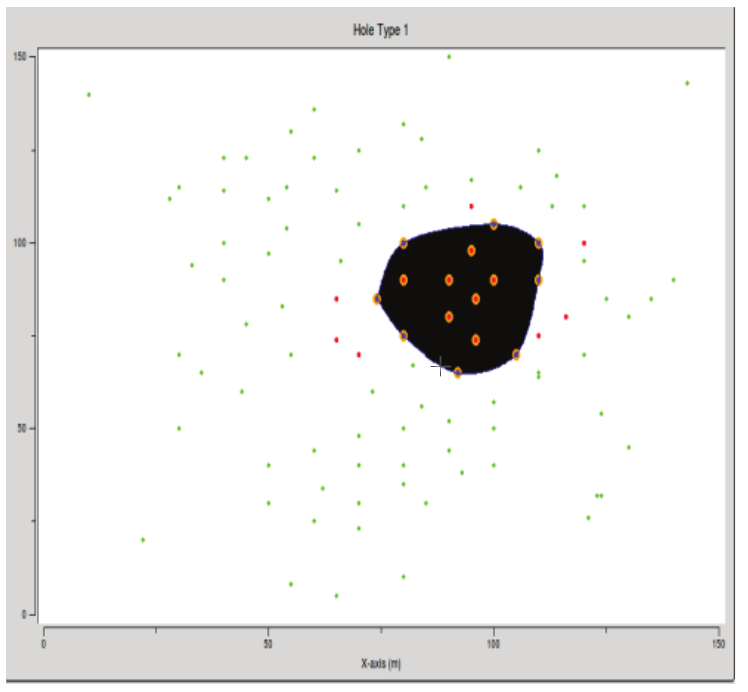
\includegraphics[width=0.8\linewidth]{arya2015_kuva}
  \caption{Simulaatiokuva artikkelissa~\cite{Arya2015} määritellystä
algoritmista. Kuvassa näkyy anturien kuolemasta syntynyt reikä mustalla.}
\label{fig:arya2015}
\end{figure}

